\documentclass[xcolor=pdftex,dvipsnames]{beamer}
\usepackage{harvard}
\usepackage{amsmath}
\usepackage{amssymb}
\usepackage{comment}
\usepackage{textcomp}


\title{Microeconomic Theory --- ECON 323 503 \\ Chapter 2: Supply and Demand} 
\author{Vikram Manjunath}
\institute{Texas A\&M University}
\setbeamertemplate{navigation symbols}{}
\setbeamertemplate{footline}{}
\usefonttheme{serif}
\begin{document}



\maketitle

\begin{frame}
\frametitle{Outline}
\begin{enumerate}[<+->]
\item Demand: How much do consumers want to buy at a particular price?
\item Supply: How much do firms want to sell at a particular price?
\item Market Equilibrium: Interaction between the two.
\item Comparative statics: Effects of small changes in the environment.
\item Elasticity: A handy description of supply or demand.
\end{enumerate}
\end{frame}


\begin{frame}
\frametitle{Outline}
\begin{enumerate}[<+->]
\item[6.] Effects of a sales tax.
\item[7.] When supply $\neq$ demand.
\item[8.] When to (and not to) use this model.
\end{enumerate}
\end{frame}


\begin{frame}
\frametitle{Demand}
How much of something do consumers want at a particular price?\bigskip

\uncover<2->{
Depends on (among other things):
\begin{enumerate}
\item Information
\item Prices of other things
\item Income
\item Regulations
\end{enumerate}
}
\end{frame}


\begin{frame}
\frametitle{Demand Function}
Demand is a function of the  price of the good  and all of those other things.\bigskip

\uncover<2->{Can, for instance, write the following:
\[
Q=D(p,p_s,p_c,Y)
\]
where
\begin{itemize}
\item $p$ is the price of the good that we're studying.
\item $p_s$ is the price of a ``substitute good.''\item $p_c$ is the price of a ``complementary good.''\item $Y$ is the consumer's income.
\end{itemize}}
\end{frame}


\begin{frame}
\frametitle{An example}
The Canadian Pork market.
\[
Q = 171 - 20p +20p_b + 3p_c +2Y
\]
where 
\begin{itemize}
\item $p$ is the price of pork (\$/kg).
\item $p_b$ is the price of beef (a substitute) (\$/kg).
\item $p_c$ is the price of chicken (another substitute) (\$/kg).
\item $Y$ is the consumer's income (thousand \$/year).
\end{itemize}


\end{frame}

\begin{frame}
\frametitle{An example}

Suppose we know that  $p_b=\$4, p_c=\$3\frac{1}{3},$ and $Y=12.5$
\bigskip


\uncover<2->{
Then, 
\[Q=286-20p = D(p).\]
}

\end{frame}



\begin{frame}
\frametitle{Graphically}
The \emph{demand curve}:

\begin{center}
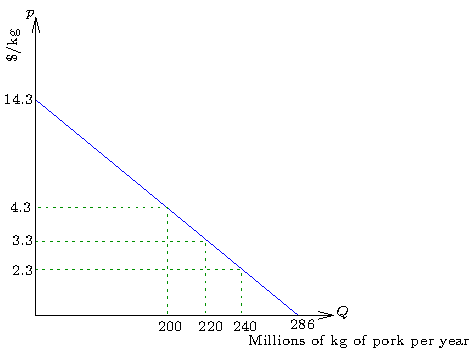
\includegraphics{pics/DemandCurve}
\end{center}

Convention: $p$ on the vertical and $Q$ on the horizontal axis.
\end{frame}


\begin{frame}
\frametitle{What happens when the price changes?}
As the price increases, quantity demanded decreases.

\bigskip
\uncover<2->{
This is the {\color{red} Law of Demand}. \bigskip
}


\uncover<3->{
Two equivalent ways to say this:
\begin{enumerate}
\item The demand curve slopes downwards.
\item $\frac{dQ}{dp}<0$.
\end{enumerate}\bigskip
}

\uncover<4->{
But we move \emph{along} the demand curve.
}

\end{frame}






\begin{frame}
\frametitle{What if other things change?}
Changes in prices of other goods, income, regulations, etc. affect the quantity demanded.
\bigskip

They cause the entire demand curve to shift up or down.
\end{frame}





\begin{frame}
\frametitle{Pork example}
Suppose that the price of beef rises to \$4.60 a kg.

\uncover<2->{
New demand curve is given by 
\[
D(p) = 298-20p.
\]
}

\uncover<3->{
What happened to its slope?
}
\uncover<4->{ It didn't change.}

\bigskip
\uncover<5->{But the curve itself shifted upwards: if beef is more expensive, people buy more pork.
}


\end{frame}



\begin{frame}
\frametitle{Graphically}
\begin{center}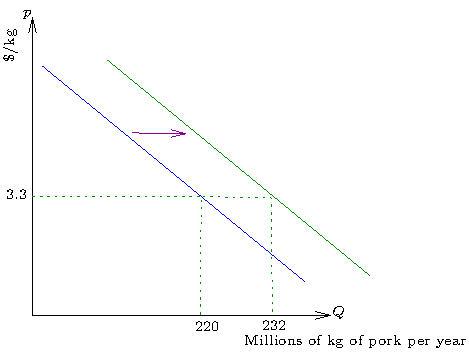
\includegraphics{pics/DemandShift}\end{center}
\end{frame}



\begin{frame}
\frametitle{Summing Demand Functions}
Suppose that Ann's demand function is $D_A$ and Bob's demand function is $D_B$. What is their total demand?

\uncover<2->{Just add them up:
\[
Q=Q_A + Q_B = D_A(p) + D_B(p).
\]
}
\end{frame}



\begin{frame}
\frametitle{Summing Demand Curves}
We add the demand curve horizontally.

\begin{center}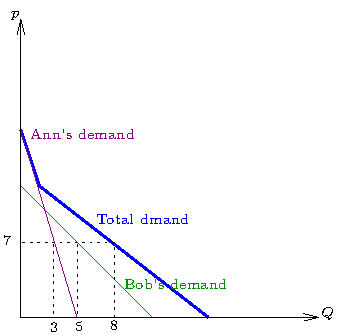
\includegraphics{pics/DemandSum}
\end{center}
\end{frame}





\begin{frame}
\frametitle{Supply }
How much of something do firms want to sell at a particular price?\bigskip

\uncover<2->{
Depends on
\begin{enumerate}\item Production costs
\item Regulations
\end{enumerate}
}
\end{frame}




\begin{frame}
\frametitle{Supply function}
Supply is a function of the price of the good as well as the prices of inputs.\bigskip

\uncover<2->{Sticking with the pork example,
\[
Q=S(p,p_h)
\]
where $p_h$ is the price of hogs (\$/kg).
}\bigskip

\uncover<3->{
Based on one study, 
\[
Q=178+40p-60p_h.
\]
}
\uncover<4->{
If $p_h=1.5$,
\[
Q=88+40p.
\]
}


\end{frame}



\begin{frame}
\frametitle{Graphically}
The \emph{supply curve}:
\begin{center}
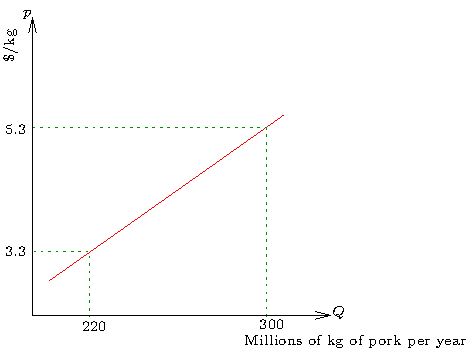
\includegraphics{pics/SupplyCurve}
\end{center}
\end{frame}


\begin{frame}
\frametitle{Changes}
Changes in the price: Typically supply increases with the price (but there's no ``Law of Supply''). Movement is \emph{along} the supply curve.\bigskip

\uncover<2->{
Changes in other things: In our example, the price of hogs could change. This would shift the entire supply curve.\bigskip
}

\uncover<3->{If the price of hogs increases to \$1.75,
\[
Q=73+40p
\]
Since the price of hogs goes up, the supply curve shifts left: If hogs
are more expensive, firms need a higher price to supply the same
amount of pork.
\bigskip

}

\end{frame}

\begin{frame}
\frametitle{Shifting supply curves}

\begin{center}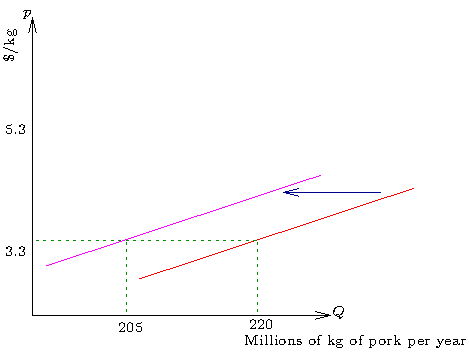
\includegraphics{pics/SupplyShift}
\end{center}
\end{frame}


\begin{frame}
\frametitle{Summing Supply Functions}
$S^D$: Japanese domestic supply of rice.\bigskip

$S^F$: Foreign supply of rice.

Total supply is just
\[
Q=Q^D + Q^F = S^D(p)+S^F(p).
\]

\uncover<2->{
One way the government could affect the total supply is by choosing to ban imports. Then the total supply would be described by $S^D$ rather than $S^D+S^F$.
}
\end{frame}


\begin{frame}
\frametitle{Market Equilibrium}
You've heard it a million times:
\begin{center}
\emph{\color{red} Demand equals supply.}
\end{center}\bigskip

\uncover<2->{
This is the concept of an equilibrium: no participant wants to change his behavior.\bigskip

Consumers want to buy the same quantity that firms want to sell.
}
\end{frame}

\begin{frame}
\frametitle{Where is the equilibrium?}
\begin{center}
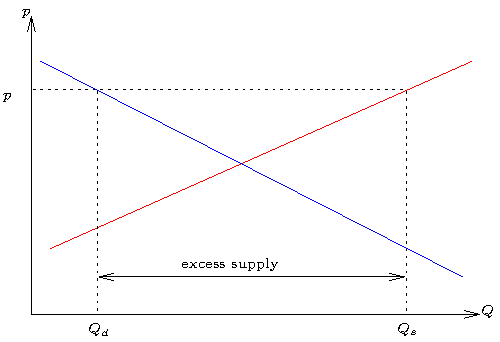
\includegraphics{pics/Equilibrium0}
\end{center}
\end{frame}

\begin{frame}
\frametitle{Where is the equilibrium?}
\begin{center}
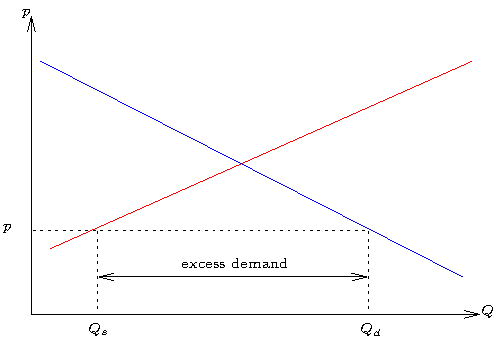
\includegraphics{pics/Equilibrium01}
\end{center}
\end{frame}

\begin{frame}
\frametitle{Where is the equilibrium?}
\begin{center}
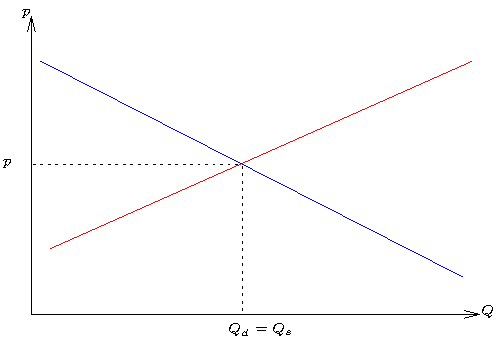
\includegraphics{pics/Equilibrium02}
\end{center}
\end{frame}

\begin{frame}
\frametitle{An example}
\[
\begin{array}{rcl}
Q_d &=& 286-20p\\
Q_s&=&88+40p
\end{array}
\]

Need to find$p$ where $Q_d=Q_s$.\bigskip

\uncover<2->{
Setting $Q_d=Q_s$:
\[
286-20p = 88+40p.
\]
So we find that $p=\$3.30$.
}

\end{frame}


\begin{frame}
\frametitle{How do we get to equilibrium?}

Every actor behaves independently. Yet we get to an equilibrium. How?
\bigskip

\uncover<2->{Adam Smith's \emph{invisible hand} is how.}\bigskip

\uncover<3->{
If the price is too high, sellers can't find enough buyers.

They'd have to dispose (or store) their wares and incur a cost. This
would lead to a change in their choice of how much to supply. \bigskip

}
\uncover<4->{
If the price is too low, buyers can't find enough sellers.

Some buyers would offer more than that price to get what they want.  \bigskip
}

\uncover<5->{ When the price is \emph{just} right, nobody changes
  their behavior.}
\end{frame}

\begin{frame}\frametitle{Comparative statics}
Compare what happens before and after a change to something in the
environment, like a change in the price of hogs.\bigskip

\uncover<2->{
Suppose the price of hogs increases from \$1.50 to \$1.75.

What is the effect on the equilibrium?
}
\bigskip

\uncover<3->{
Original equilibrium price was \$3.30 with consumers demanding 220
million kg. But supply is only 205. The price is too low.\bigskip
}

\uncover<4->{Equating supply and demand, we find the new equilibrium
  price of \$3.55 and quantity of 215 million kg.\bigskip
}

\uncover<5->{So the increase in $p_h$ cause and increase in the
  equilibrium price and a decrease in the equilibrium quantity.}


\end{frame}

\begin{frame}\frametitle{Small changes}
Here, we can use some calculus so that we don't have to actually
calculate and recalculate the equilibrium.\bigskip

\uncover<2->{Suppose supply depends on the environmental variable $a$:
\[
S(p,a).
\]
Demand doesn't: $D(p)$. \bigskip}

\uncover<3->{Equilibrium price solves 
\[
S(p,a)=D(p).
\]


This solution is a function of $a$. Call it $p(a)$.\bigskip}


\uncover<4->{So, the equilibrium condition is actually
\[
S(p(a),a) = D(p(a)).
\]
}



\end{frame}



\begin{frame}
\frametitle{Small changes}
Using the ``chain rule'':
\[
\frac{dD(p(a))}{dp}\frac{dp}{da} = \frac{\delta S(p(a),a)}{\delta
  p}\frac{dp}{da} + \frac{\delta S(p(a),a)}{\delta a}.
\]

\uncover<2->{
Rearranging this:
\[
\frac{dp}{da} = \dfrac{\frac{\delta S}{\delta a}}{\frac{dD}{dp} -
  \frac{\delta S}{\delta p}}.
\]}
\uncover<3->{
Since $\frac{dD}{dp}<0$, if $\frac{\delta S}{\delta p} >0$, then
$\frac{dp}{da}$ has the opposite sign as $\frac{\delta S}{\delta a}$.
}\bigskip

\uncover<4->{
We can also differentiate $Q=D(p(a)$ to see that 
\[
\frac{dQ}{da} = \frac{dD}{dp}\frac{dp}{da}.
\]
}
\uncover<5->{
Since $\frac{dD}{dp}<0$,$\frac{dQ}{da}$ has the opposite sign as $\frac{dp}{da}.$
}
\end{frame}

\begin{frame}
\frametitle{How big are the changes?}
The comparative statics that we just saw usually tell us the sign of
the effect. But the magnitude depends on the shape of the supply and
demand curves. 
\bigskip


Say the supply curve shifts left.

\only<1>{\vspace{2.43in}}

\only<2>{
\begin{center}
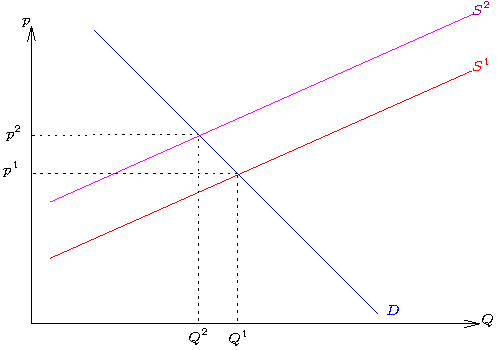
\includegraphics[scale=0.8]{pics/magn3}
\end{center}
$Q$ decreases and $p$ increases.
}



\only<3>{

\begin{center}
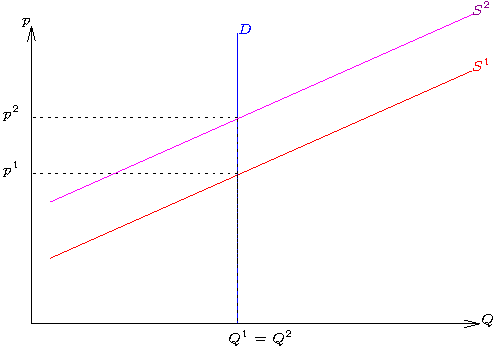
\includegraphics[scale=0.8]{pics/magn1}
\end{center}

Steeper the demand curve, smaller the change.
}
\only<4>{

\begin{center}
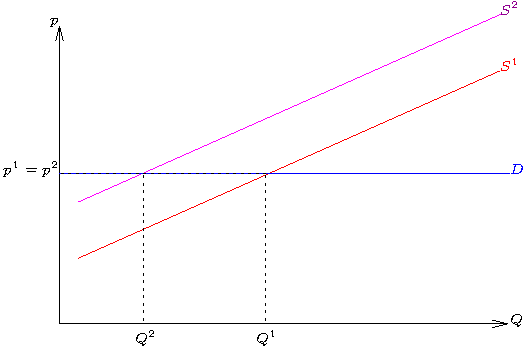
\includegraphics[scale=0.8]{pics/magn2}
\end{center}

Flatter the demand curve, bigger the change.
}
\end{frame}

\begin{frame}
\frametitle{Elasticity}
How does demand respond to a change in the price?
\bigskip

\uncover<2->{
The Law of Demand says that it decreases. \bigskip
}

\uncover<3->{
But is there a nice way to summarize by how much?\bigskip
}

\uncover<4->{
Elasticity of demand: percentage change in demand for a 1\% change in
price:
\[
\varepsilon=\dfrac{\frac{\Delta Q}{Q}}{\frac{\Delta P}{P}}
=\frac{\delta Q}{\delta p}\frac{p}{Q}.
\]
}
\uncover<5->{
If $\varepsilon=-2$, then a 1\% increase in price leads to a -2\%
increase in demand (or, more reasonably, a 2\% decrease).
}
\end{frame}

\begin{frame}
\frametitle{Calculating elasticity}
\[
Q=a-bp
\]
\uncover<2->{
\[
\varepsilon = \frac{dQ}{dp}\frac{p}{Q} = -b\frac{p}{Q}
\]
}

\uncover<3->{
For our pork example, $a=286$ and $b=20$ so at $p=\$3.30$ and $Q=220$,
$\varepsilon=-20\times \frac{3.30}{220}=-0.3$
}
\end{frame}


\begin{frame}
\frametitle{Moving along the demand curve}
What happens to elasticity as we move along the demand curve?

\uncover<2->{
For the demand curve we just saw, it depends on $p$ and
$Q$.\bigskip
}

\uncover<3->{
If $p=0$, then $\varepsilon=0$: demand is \emph{perfectly inelastic}.
Changes in price don't affect demand any further.\bigskip
}

\uncover<4->{
If $Q=0$, then $\varepsilon=-\infty$: demand is \emph{perfectly elastic}.
Any increase in price drops demand to zero.\bigskip
}

\end{frame}
\begin{frame}
\frametitle{Moving along the demand curve}

Moving between these two extreme points we have every possible value
between 0 and $-\infty$.

\uncover<2->{
\emph{Unitary elasticity}: $\varepsilon=-1$. The percentage change in
demand is the same as the percentage change in price.

This happens when $p=\frac{a}{2b}$ and $Q={a}{2}$\bigskip
}


\uncover<3->{
\emph{Elastic demand}: $\varepsilon<-1$. The percentage change in
demand is more than the percentage change in price.

This happens to the left of unitary elasticity. \bigskip
}

\uncover<4->{
\emph{Inelastic demand}: $\varepsilon>-1$. The percentage change in
demand is less than the percentage change in price.

This happens to the right unitary elasticity.\bigskip
}
\end{frame}
\begin{frame}
\frametitle{Moving along the demand curve}
\begin{center}
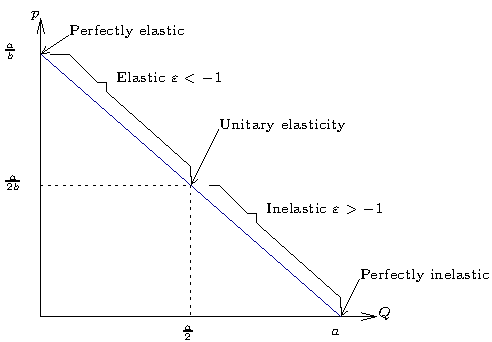
\includegraphics{pics/Elast}
\end{center}
\end{frame}



\begin{frame}
\frametitle{Can elasticity be constant?}

\[
Q=Ap^\varepsilon
\]

Elasticity is $\varepsilon$ no matter $p$ and $Q$.
\bigskip

\uncover<2->{
If the demand curve is a horizontal line, demand is perfectly elastic everywhere.

This happens when a good has a perfect substitute: if the price rises,
everyone just switches to the other good.
}
\bigskip

\uncover<3->{
If the demand curve is a vertical line, demand is perfectly inelastic everywhere.

This happens when a good is \emph{essential}: you can't live without~it.
}


\end{frame}

\begin{frame}
\frametitle{Other demand elasticities}
What we saw is actually called the ``price elasticity'' of demand.
\bigskip

But we can just as well define 
\begin{enumerate}[<+->]
\item Income elasticity: percentage change in demand for a 1\% increase
  in income.
\item Cross-price elasticity: percentage change in demand for a 1\% increase
  in the price of another good. This is relevant for substitutes and
  complements.
\end{enumerate}
\end{frame}

\begin{frame}
\frametitle{Supply elasticity}
\[
\eta =\dfrac{\text{\% change in supply}}{\text{\% change in price}} =
  \dfrac{\frac{\Delta Q}{Q}}{\frac{\Delta p}{p}} = \frac{\delta
    Q}{\delta p}\frac{p}{Q}.
\]

\uncover<2->{
For the Pork example: $Q=88+40p$ so at $p=\$3.30$ and $Q=220$,

\[
\eta =  \frac{\delta
    Q}{\delta p}\frac{p}{Q} = 40\times \frac{3.30}{220} =0.6.
\]
}

\uncover<3->{
Unlike demand elasticity, supply elasticity is positive
valued (except in the rare case where the supply curve slopes downwards).
}
\end{frame}


\begin{frame}\frametitle{Moving along the supply curve}
Elasticity varies along the supply curve: it depends on $\frac{p}{Q}$.\

\uncover<2->{
\begin{itemize}
\item $\eta=0$: perfectly inelastic supply.
\item $0<\eta<1$: inelastic supply.
\item $1<\eta$: elastic supply
\item $\eta=\infty$: perfectly elastic supply.
\end{itemize}

}

\end{frame}

\begin{frame}\frametitle{Elasticity over time}
Whether elasticity is greater over the long or short run depends on
how easily the good is replaced.

\uncover<2->{\begin{itemize}
\item An electric car isn't a good substitute for a gas car in the
  short run, but it is in the long run.
\item A mac is a good substitue for a PC in the short run, but once
  you get ``locked in'' it's not a good substitute.
\end{itemize} }

\uncover<3->{
The easier it is to substitute a good, the more elastic demand will be.\bigskip
}


\uncover<4->{Similar reasoning applies to supply elasticity.}
\end{frame}


\begin{frame}
\frametitle{Effects of a sales tax}
Two types of tax: 
\begin{enumerate}
\item \emph{Ad valorem} tax: a percentage of the sales price. If the
  price of an apple is $p$, you pay $(1+\alpha)p$ where $\alpha$ is
  the tax rate. This is the most common form.
\item \emph{Unit or specific} tax: the tax doesn't depend on the sales price. If
  the price of an apple is $p$, you pay $p+\tau$ where $\tau$ is the
  tax rate. E.g. federal tax on gasoline.
\end{enumerate}
\end{frame}



\begin{frame}
\frametitle{Effect of tax on equilibrium}
Specific tax: $\tau$.
\bigskip

\uncover<2->{
Consumer pays $p$ $\longrightarrow$ $\tau$ to government  and
$p-\tau$ to supplier.\bigskip
}

\uncover<3->{
Since supplier only gets $p-\tau$ at price $p$, supply curve shifts left.
}


\end{frame}
\begin{frame}
\frametitle{An example}
Canadian pork:
Suppose $\tau=\$1.05$ per kg. 

\bigskip\uncover<2->{Without tax: at price \$2.95, supply of 206 million kg.}

\bigskip
\uncover<3->{After tax, supplier only gets \$1.90 so the supply is less.}

\bigskip

\uncover<4->{At what price does the firm supply 206 million kg? Needs to receive
\$2.95, so price needs to be \$2.95+$\tau$ = \$4.00.}

\bigskip
\uncover<5->{Supply curve shifts  left (up) by $\tau$.}
\bigskip

\uncover<6->{Equilibrium price goes up, equilibrium quantity goes down.}
\bigskip

\uncover<7->{We'll see that the elasticity determines by how much.}
\end{frame}


\begin{frame}
\frametitle{Graphically}
\only<1>{
\begin{center}
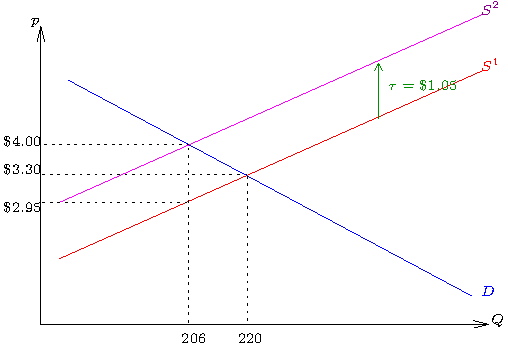
\includegraphics{pics/TaxEffect1}
\end{center}
}
\only<2>{
\begin{center}
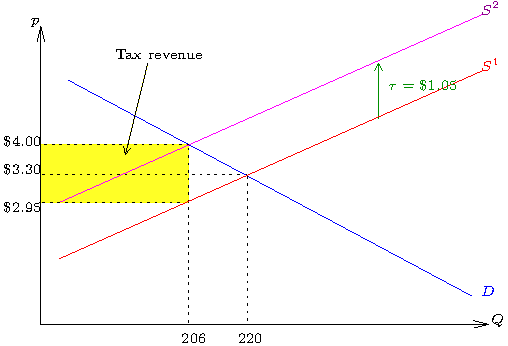
\includegraphics{pics/TaxEffect2}
\end{center}
}
\uncover<2>{
Tax revenue = $\tau Q$= \$216.3 million.
}

\end{frame}


\begin{frame}
\frametitle{Who's really paying the tax?}
What we want to know is this: how much does the \emph{price} change
because of the tax? In the example, price only changed by \$0.70=\$4.00 -
\$3.30 even though tax was \$1.05.

\bigskip\uncover<2->{
 What we really want is: $\frac{dp}{d\tau}$.
}

\bigskip\uncover<3->{

Equilibrium condition \emph{with} tax:
\[
D(p) = S(p-\tau).
\]}

\uncover<4->{
The equilibrium price is a function of the tax: $p(\tau)$.
 So we can write the equilibrium condition as 
\[D(p(\tau)) = S(p(\tau)-\tau).
\]
}


\end{frame}


\begin{frame}
\frametitle{Who's really paying the tax?}
Differentiating this with respect to $\tau$
\[
\frac{dD}{dp}\frac{dp}{d\tau} =
\frac{dS}{dp}\frac{d(p(\tau)-\tau)}{d\tau} = \frac{dS}{dp}\left(\frac{dp}{d\tau}-1\right).
\]
\uncover<2->{
Rearranging this,
\[
\frac{dp}{d\tau}
=\dfrac{\frac{dS}{dp}}{\frac{dS}{dp}-\frac{dD}{dp}}.
\]
}
\uncover<3->{
We know the sign of this: $\frac{dD}{dp} <0$ and $\frac{dS}{dp} > 0$
so $\frac{dp}{d\tau}>0$. This means that the price increases with tax.
}

\bigskip\uncover<4->{
The exact rate at which it increases depends on elasticities:
Multiplying numerator and denominator by $\frac{p}{Q}$,
\[\frac{dp}{d\tau}
=\dfrac{\frac{dS}{dp}\frac{p}{Q}}{\frac{dS}{dp}\frac{p}{Q}-\frac{dD}{dp}\frac{p}{Q}}
= \frac{\eta}{\eta-\varepsilon}.
\]}

\end{frame}

\begin{frame}
\frametitle{Who's really paying the tax?}
Now we can really answer this question:

\begin{enumerate}
\item \emph{Incidence of tax on consumers:} $\frac{dp}{d\tau}$.
\item \emph{Incidence of tax on suppliers:} $1-\frac{dp}{d\tau}$.
\end{enumerate}
\end{frame}

\begin{frame}
\frametitle{What if we made the consumers pay instead of the
  suppliers?}
Again, specific tax: $\tau$.\bigskip

Consumer pays $p+\tau\to \tau$ to government and $p$ to supplier
\bigskip

Supplier gets $p$.\bigskip

Since, at price $p$, consumer pays $p+t$, demand curve shifts down.
\bigskip

Equilibrium condition is 
\[
D(p+\tau) = S(p).
\]
For the pork example solving this, $p=\$2.95$. \bigskip

\uncover<2->{
Nothing changed! The consumer still pays \$4($=p+\tau$).
}
\end{frame}
\begin{frame}
\frametitle{Consumers paying the tax}
\begin{center}
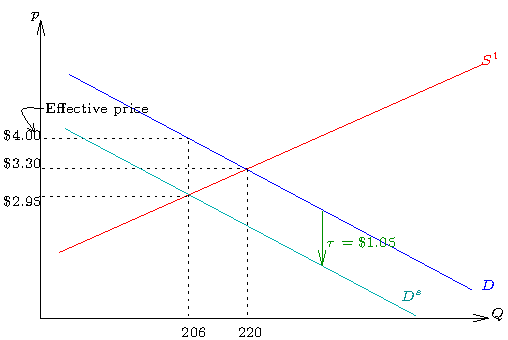
\includegraphics{pics/DemandTax1}
\end{center}
\end{frame}
\begin{frame}
\frametitle{What about \emph{ad valorem} tax?}
The tax that consumers pay per unit is $\alpha=\frac{\tau}{p} =
\frac{1.05}{3.30} =26.25\%$.
\bigskip

\uncover<2->{What if we replaced the specific tax $\tau$ with an ad valorem tax~$\alpha$?}\bigskip

\uncover<3->{The demand curve $D^a$ would rotate, gap between $D$ and
  $D^a$ being $\alpha p$.
}

\end{frame}
\begin{frame}
\frametitle{Graphically}
\begin{center}
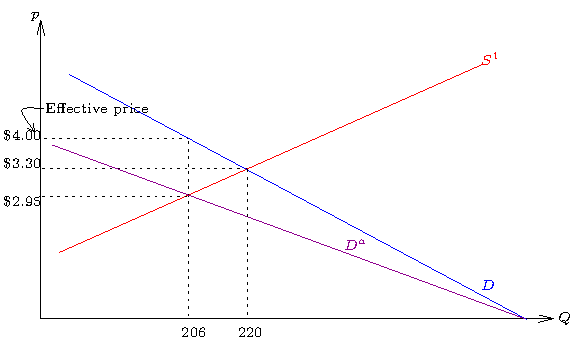
\includegraphics{pics/DemandTax2}
\end{center}
\end{frame}
\begin{frame}
\frametitle{Ad valorem vs unit tax}
\begin{center}
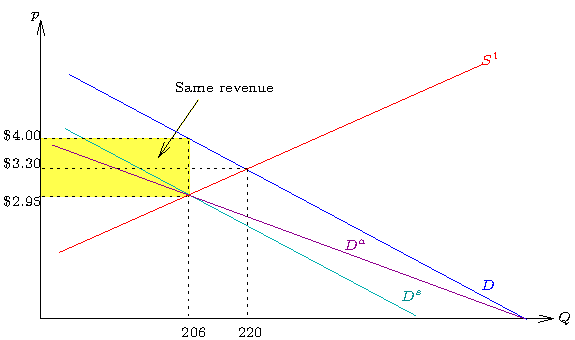
\includegraphics{pics/DemandTax3}
\end{center}
\end{frame}

\begin{frame}
\frametitle{When supply $\neq$ demand}
Sometimes, demand (what consumers \emph{want to
  buy} at a particular price) and supply (what firms \emph{want to
  sell} at a particular price) may differ.
\bigskip

This may happen because of certain kinds of government interventions
like price controls.

\begin{enumerate}
\item Price ceiling: price is legally required to be below a certain 
  threshold  $\overline p$. Example: gas prices in the 1970s, rent
  control in NYC.
\item Price floor: price is legally required to be above a certain 
  threshold  $\overline p$. Example: minimum wage
\end{enumerate}
\end{frame}






\begin{frame}
\frametitle{Example of price ceiling}

Oil supply is reduced: supply curve shifts left.

Equilibrium price goes from $p_1=\$5$ to $p_2=\$6$.

Government outlaws a price increase: prices cannot exceed $\overline
p=\$5$.

Does quantity demand equal quantity supplied?


\end{frame}
\begin{frame}
\frametitle{Gasoline price ceiling}
\begin{center}
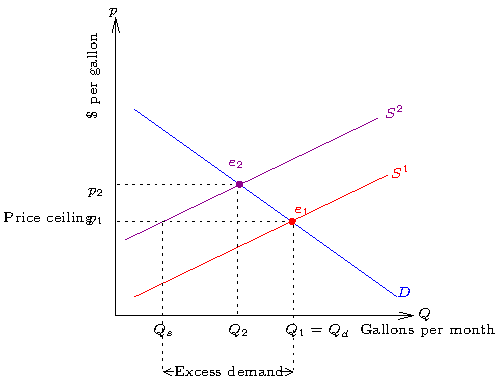
\includegraphics{pics/GasCeiling}
\end{center}
\end{frame}

\begin{frame}
\frametitle{When to use this model}
Some key assumptions (limitations) of the model:
\begin{enumerate}[<+->]
\item There are many identical firms and consumers: nobody can affect
  the price on their own.
\item Everyone has full information: everyone knows all prices and
  characteristics of goods.
\item There are no transaction costs.
\item Firms can easily enter and exit the market.
\end{enumerate}

\end{frame}

\begin{frame}
\frametitle{When to use this model}
These assumptions actually \emph{seldom} hold in reality. Examples of violations:
\begin{enumerate}[<+->]
\item Small/identical firms and consumers: utilities, artists
\item Full information: used cars
\item There are no transaction costs: broker's fees
\item Firms can easily enter and exit the market: almost all manufacturing
\end{enumerate}

\end{frame}


\begin{frame}
\frametitle{Solution of  problem 5.8 from the textbook}
Demand function for coconut oil:
\[
Q=1,200-9.5p+16.2 p_p + 0.2Y
\]
where \\
\begin{tabular}{lcl}
$Q$ & ---& Quantity demanded (1,000s of metric tons)\\
$p$ & ---& price of coconut oil (\textcent/lb)\\
$p_p$ & ---& price of palm oil  (\textcent/lb)\\
$Y$  & ---& consumer's income
\end{tabular}\bigskip

Calculate price and cross-price elasticity of the demand for coconut
oil at $p=45$\textcent/lb,  $p_p=31$\textcent/lb, and $Q=1,275$
thousand metric tons.
\end{frame}


\begin{frame}
\frametitle{Solution of  problem 5.8: price elasticity}
\begin{enumerate}[<+->]
\item Express demand as a function of $p$:
Substituting value of $p_p$
\[
Q=1,200-9.5p + 16.2\times 31 +0.2Y = {\color{red}1702.2 + 0.2 Y - 9.5p}
\]
\item So $\frac{dQ}{dp} = -9.5$
\item $\varepsilon=\frac{dQ}{dp}\frac{p}{Q} = (-9.5)\times\frac{45}{1,275}
  \approx -0.34 $.
\end{enumerate}
\uncover<4->{
So a \underline{1\% increase} in the price of coconut oil leads to about a
\underline{0.34\% decrease} in demand for it.
}
\end{frame}
\begin{frame}
\frametitle{Solution of  problem 5.8: cross-price elasticity}
\begin{enumerate}[<+->]
\item Express demand as a function of $p_p$:
Substituting value of $p$
\[
Q=1,200-9.5\times 45 + 16.2p_p +0.2Y = {\color{red}772.5 + 0.2 Y + 16.2p_p}
\]
\item So $\frac{dQ}{dp_p} = 16.2$
\item $\varepsilon=\frac{dQ}{dp}\frac{p}{Q} = 16.2\times
  \frac{31}{1,275} \approx 0.39$.
\end{enumerate}
\uncover<4->{
So a \underline{1\% increase} in the price of palm oil leads to about a
\underline{0.39\% increase} in demanded for coconut oil.
}
\end{frame}
\end{document}